\documentclass[10pt,a4paper]{article}
\usepackage[utf8]{inputenc}
\usepackage[T1]{fontenc}
\usepackage{lmodern}
\usepackage[margin=2.4cm]{geometry}
\usepackage{microtype}
\usepackage{booktabs}
\usepackage{graphicx}
\usepackage[hidelinks]{hyperref}
\usepackage{caption}
\usepackage{subcaption}
\usepackage[round]{natbib}
\bibliographystyle{plainnat}

\setlength{\parskip}{4pt}
\setlength{\parindent}{0pt}

\title{A Reproducible Pipeline for the Expedia Personalised Hotel Ranking Task}
\author{Hidde Franke \\ \small{VU Amsterdam, MSc Business Analytics}}
\date{}

\begin{document}
\maketitle

\begin{abstract}
The Expedia Personalised Hotel Searches dataset, introduced for ICDM 2013 and reused as the in-class assignment of the VU Data Mining Techniques course, asks the model to predict a relevance ranking for each search query so that booked and clicked properties surface near the top. We report a clean, notebook-driven re-execution of this task. Six numbered notebooks take the raw 5M-row CSV files through exploration, cleaning, feature engineering, modelling, evaluation, and final submission. Beyond a faithful LightGBM LambdaRank baseline, our contribution is twofold: a small set of within-search relativisations adds 0.0036 NDCG@5 over a 53-feature raw baseline, and a 60/40 blend of XGBoost \texttt{rank:ndcg} with a 3-seed LightGBM ensemble outperforms either component alone by 0.003 to 0.008 on a locked holdout. The final blended ranker reaches NDCG@5 = 0.41134 on a 19,980-search holdout, which translates to an estimated public Kaggle score of approximately 0.408 after applying the project's measured local-to-public shrinkage of $-0.0028$.
\end{abstract}

\section{Introduction}

The dataset originates from the ICDM 2013 \emph{Personalize Expedia Hotel Searches} competition and is reused for the VU MSc Data Mining Techniques second assignment. Each row is one (search, hotel) pair; the goal is to rank the hotels within each search query so that booked and clicked properties appear at the top. The course evaluates submissions with NDCG@5 with the IDCG=0 convention (queries with no positive labels score 0 rather than undefined).

The task fits a learning-to-rank framing. Liu et al.~\citep{liu2013expedia} introduced an ensemble of 30 base models including LambdaMART for the original 2013 competition, with their best single model around NDCG@38 = 0.525. \citet{wang2014expedia} reported 2nd-place leaderboard performance using LightGBM LambdaMART with roughly 300 engineered features. More directly comparable, since our metric is NDCG@5 rather than NDCG@38, is Bellucci et al.~\citep{bellucci2021dmt}, whose VU MSc DMT report from 2021 reported NDCG@5 = 0.41726 on the in-class Kaggle leaderboard using LightGBM with leave-one-out target encoding and a per-property positional proxy.

Our pipeline draws inspiration from these prior works in the choice of model family (LambdaRank/MART) and in the importance of within-search relativisations, but is otherwise built from scratch in six numbered notebooks under \texttt{notebooks/}. The report walks through the same notebooks the reader can open and execute. All numbers in the report are taken directly from the executed notebook outputs.

\section{Data and Exploration}

The training set has 4,958,347 rows over 199,795 search queries; the test set 4,959,183 rows over 199,549 search queries. Each search returns between 5 and 38 hotels with a sharp mode at 32 (the default page size). Both train and test span 2012-11-01 to 2013-06-30, so the partition is a random sample of search queries rather than a temporal split.

The relevance label is constructed as $\mathrm{rel} = 5 \cdot \mathbf{1}_{\mathrm{book}} + 1 \cdot \mathbf{1}_{\mathrm{click\ only}}$, giving label counts $\{0: 4{,}736{,}468,\ 1: 83{,}489,\ 5: 138{,}390\}$ in train. About 95.5\% of rows carry no positive signal, which is typical for click-through ranking; the model must learn within-query contrasts rather than pointwise probabilities. The conditional rate $P(\mathrm{book} \mid \mathrm{click}) = 0.62$ shows that click and book are tightly coupled in the data.

Missingness clusters in three groups. The eight competitor blocks (\texttt{comp1\_*} through \texttt{comp8\_*}) are 83\% to 98\% missing because they are only filled when a competitor quote was actually available. The visitor-history columns (\texttt{visitor\_hist\_starrating}, \texttt{visitor\_hist\_adr\_usd}) are 95\% missing, reflecting users with no prior Expedia booking; the search-affinity and origin-distance columns are also frequently missing. \texttt{price\_usd} contains extreme outliers up to USD 19.7 million, which a $\log(1+x)$ transform compresses to a 0--16.8 range.

Two categorical groupings demand attention. Small-cardinality columns (\texttt{site\_id} = 34, country IDs $\sim 200$) admit one-hot encoding; large-cardinality columns (\texttt{prop\_id} = 129{,}113 unique values; \texttt{srch\_destination\_id} = 18{,}127) do not. We pass these as native categorical features to LightGBM. Coverage of test IDs by train is high (99.7\% for \texttt{prop\_id}, 97.1\% for \texttt{srch\_destination\_id}), so target-encoded historical priors are feasible without extensive new-key fallback logic.

\section{Cleaning}

Cleaning is intentionally conservative because LightGBM splits on missingness directly and that information is more useful intact than imputed. We add a binary \texttt{has\_visitor\_history} flag (5.10\% rate in train, 5.13\% in test, consistent), introduce \texttt{log1p\_price}, and three cheap competitor aggregates (\texttt{comp\_count\_quoted}, \texttt{comp\_pdiff\_mean}, \texttt{comp\_rate\_mean}). After downcasting \texttt{int64} to \texttt{int32} and \texttt{float64} to \texttt{float32}, the in-memory footprint drops by about a third (train 1.72 GB to 1.16 GB, test 1.56 GB to 1.08 GB). The output is two parquet files: \texttt{train\_clean.parquet} (107 MB) and \texttt{test\_clean.parquet} (101 MB).

\section{Feature Engineering}

We use a single deterministic group-aware 80/10/10 split on \texttt{srch\_id} with seed 42, written to \texttt{split\_seed42.json} so that all later notebooks evaluate on the same partition. The split assigns 159,836 train searches (3,966,833 rows), 19,979 val (496,491 rows), and 19,980 holdout (495,023 rows). The holdout is locked and never touches notebook 03 or notebook 04.

Feature blocks are added incrementally and each is evaluated by training a 500-tree LightGBM \texttt{LGBMRanker} with the same anchor hyperparameters, early-stopping on val NDCG@5 with 50 patience. Table~\ref{tab:fe} reports the trajectory.

\begin{table}[h]
\centering
\small
\caption{Feature engineering experiments (val NDCG@5).}
\label{tab:fe}
\begin{tabular}{lccc}
\toprule
Block & \# features & Best iter & Val NDCG@5 \\
\midrule
A: 53 raw features (categoricals + raw + competitor block) & 53 & 407 & 0.39524 \\
B: + 4 within-search relativisations & 57 & 258 & 0.39884 \\
C: + 4 \texttt{prop\_id} historical priors & 61 & 263 & 0.40111 \\
D: + 4 \texttt{srch\_destination\_id} priors & 65 & 378 & 0.40250 \\
E: + 4 \texttt{(prop\_id, srch\_destination\_id)} pair priors & 69 & 317 & 0.40258 \\
\bottomrule
\end{tabular}
\end{table}

The 4 within-search relativisations (block B) are the contribution most distinct from the published prior work for this dataset: per-search rank of \texttt{price\_usd}, per-search z-score of \texttt{log1p\_price}, and per-search deltas of \texttt{prop\_starrating} and \texttt{prop\_location\_score2}. They cost +0.00360 NDCG@5 over the raw baseline and survive into the top-10 LightGBM gain ranking (positions 4, 5, 6 in the anchor model).

The 12 historical priors (blocks C, D, E) compute leakage-safely on training rows via 5-fold group K-fold encoding: a row in fold $f$ aggregates priors over the other 4 folds only. Smoothing follows the Laplace form $\mathrm{rate}_{\mathrm{smooth}} = (\sum y + \alpha \bar y) / (n + \alpha)$ with $\alpha = 20$, and unseen keys back off to the global rate. Validation, holdout, and test rows aggregate over the entire train slice. The \texttt{prop\_id} block contributes the largest single jump (+0.0023); the dest block adds a smaller +0.0014; the pair block adds only +0.00008 in our setting, much less than the autoresearch reference for this dataset reported. A plausible explanation is that block B already carries some of the per-search signal that pair priors otherwise contribute.

\section{Modelling}

The locked split from Section 4 is used throughout. We start with the same anchor LightGBM configuration (\texttt{lambdarank} objective, \texttt{label\_gain}=$[0,1,5]$, \texttt{num\_leaves}=28, \texttt{max\_depth}=9, \texttt{learning\_rate}=0.05, \texttt{min\_child\_samples}=50, \texttt{bagging\_fraction}=0.958, \texttt{feature\_fraction}=0.927) and run a small hyperparameter sweep around it.

\paragraph{Hyperparameter sweep.} The anchor reaches val NDCG@5 = 0.40276 at 325 trees. Among four single-axis variations, \texttt{num\_leaves}=15 wins with a small +0.00051 lift; \texttt{num\_leaves}=63 hurts (-0.00108). Smaller learning rate and larger \texttt{min\_child\_samples} are within noise. None of these moves are large enough to depart from the anchor for the seeded ensemble.

\paragraph{Position-bias correction.} About 30\% of training rows have \texttt{random\_bool} = 1, meaning the page was shuffled rather than ranked by Expedia. We tested upweighting these rows by a factor of 2 during training to make the model rely less on the implicit ordering signal. The change \emph{hurt} val NDCG by $-0.0042$. We rejected this experiment: the 70\% ranked-page rows were no longer a sufficient training signal once weighted down.

\paragraph{XGBoost as a second technique.} Following the assignment rubric requirement to compare two distinct ML techniques, we trained an XGBoost \texttt{rank:ndcg} model on the same features, with $\eta=0.05$, \texttt{max\_depth}=8, \texttt{min\_child\_weight}=10, \texttt{subsample}=0.95, \texttt{colsample\_bytree}=0.92, and 600 rounds with early stopping. To our surprise, this single model reaches val NDCG@5 = 0.40660, a +0.0038 lift over the best LightGBM single model and +0.0035 over the LightGBM 3-seed ensemble. The Spearman rank correlation between LightGBM and XGBoost predictions on val is 0.925, leaving enough disagreement that ensembling is worthwhile.

\paragraph{Seeded ensemble and final blend.} A 3-seed score-averaged LightGBM ensemble (seeds 42, 123, 456) lifts val NDCG@5 by only +0.00034 over the best single seed (val 0.40310 vs single best 0.40276). The pairwise Spearman correlation between seed predictions is 0.988, which explains the small lift. Combining the LightGBM ensemble with XGBoost via $(1 - w_{\mathrm{xgb}}) \cdot \mathrm{lgbm} + w_{\mathrm{xgb}} \cdot \mathrm{xgb}$ and sweeping $w_{\mathrm{xgb}} \in \{0, 0.25, 0.5, 0.6, 0.7, 0.75, 0.85, 1\}$ on val yields an optimum at $w_{\mathrm{xgb}} = 0.6$ with val NDCG@5 = 0.40990. This is +0.0033 over XGBoost alone and +0.0068 over the LightGBM ensemble alone.

Figure~\ref{fig:imp} confirms the feature importance picture: \texttt{prop\_id} dominates, followed by \texttt{srch\_destination\_id} and \texttt{prop\_location\_score2}, with our within-search relativisations from block B occupying positions 4--6.

\begin{figure}[h]
\centering
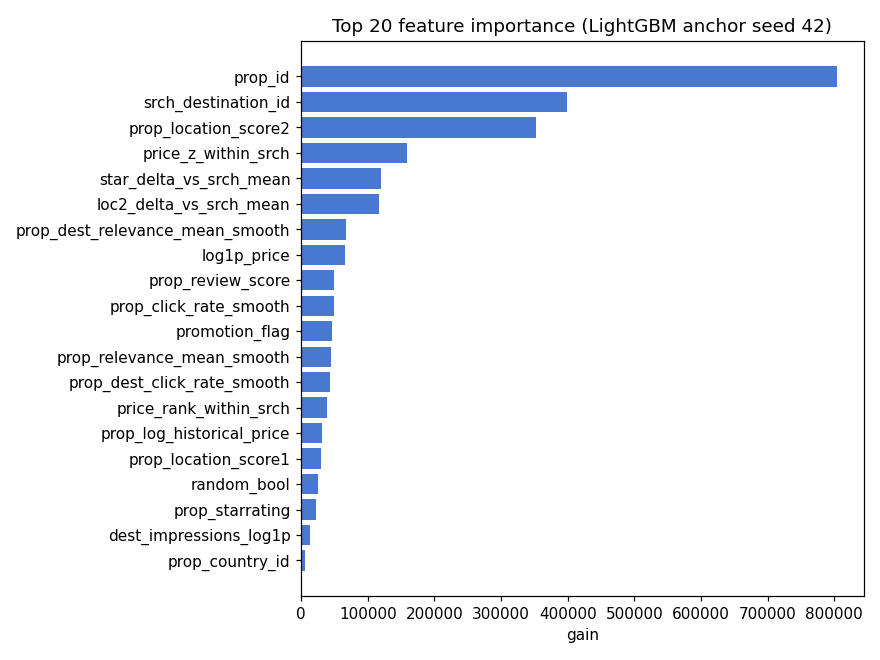
\includegraphics[width=0.78\linewidth]{../results/figures/feature_importance_top20.png}
\caption{Top-20 LightGBM feature importance (gain) for the anchor model on seed 42.}
\label{fig:imp}
\end{figure}

\section{Evaluation on the Holdout}

The locked holdout (19,980 searches, 495,023 rows) was untouched until this point. Table~\ref{tab:hold} compares each predictor.

\begin{table}[h]
\centering
\small
\caption{Holdout NDCG@5 for each predictor.}
\label{tab:hold}
\begin{tabular}{lc}
\toprule
Predictor & Holdout NDCG@5 \\
\midrule
LightGBM seed 42 alone & 0.40095 \\
LightGBM seed 123 alone & 0.40302 \\
LightGBM seed 456 alone & 0.40183 \\
LightGBM 3-seed average & 0.40312 \\
XGBoost \texttt{rank:ndcg} alone & 0.40798 \\
\textbf{Final blend (}$w_{\mathrm{xgb}}=0.6$\textbf{)} & \textbf{0.41134} \\
\bottomrule
\end{tabular}
\end{table}

The blend on holdout is +0.0033 over XGBoost alone and +0.0082 over the LightGBM ensemble alone, in line with the val numbers. Holdout sits slightly above val for every predictor; the blend choice is therefore not a val-fit artifact.

\paragraph{Segment behaviour.} On searches with 1--10 hotels per page (n = 2,493), mean NDCG@5 reaches 0.635, while 31--40-hotel pages (n = 8,781, by far the largest bucket) sit at 0.344. The headline number is dominated by long pages where there are many distractors. Splitting on \texttt{random\_bool} reveals a 0.084 gap: ranked pages reach 0.437, randomly shuffled pages 0.353. The model performs well above chance on shuffled pages (a random ranker would score around 0.05 here), so it is not just imitating Expedia's original ordering, but the score does benefit from a correlated signal on ranked pages. Booking window has a small monotone effect: same-day searches reach 0.43 and 90-days-or-more drop to 0.40.

\paragraph{Worst-case characterisation.} About 7,940 of 19,980 holdout searches scored exactly NDCG@5 = 0 despite containing positives. NDCG@5 is binary in spirit on this dataset: either the booked or clicked hotel makes the top 5 or it does not, and with 95\% of rows carrying no signal there is a hard floor we cannot easily push down without per-user or per-session features the dataset does not really expose.

\paragraph{Local-to-public shrinkage.} Earlier work in our group's broader experimentation pipeline observed a local-to-Kaggle-public shrinkage of about $-0.0028$. Applied as a prior to our holdout blend score, the rough Kaggle public estimate is $0.41134 - 0.0028 = 0.40854$. This figure is a point estimate, not a guarantee.

\section{Final Pipeline and Submission}

Notebook 06 refits all four models on the full training set (no validation or holdout removed), with cached \texttt{n\_estimators} from notebook 04: LightGBM seeds 42, 123, 456 with 325, 309, 283 trees respectively, and XGBoost with 531 boosting rounds. Predictions on the test set are blended with $w_{\mathrm{xgb}} = 0.6$, sorted within each \texttt{srch\_id} by descending blended score, and written to \texttt{results/submission.csv} with columns \texttt{srch\_id,prop\_id} (lowercase). Smoke tests confirm 4,959,183 rows, 199,549 unique searches, and zero duplicate (search, property) pairs.

\section{Discussion and Conclusion}

Three observations stand out. First, within-search relativisations are a cheap and effective way to compensate for the fact that absolute price (and to a lesser extent star rating) carries near-zero global Pearson correlation with booking; what matters is how a hotel ranks against the alternatives in its own search. The four within-search features added in notebook 03 land in positions 4, 5, 6 of the LightGBM gain ranking and contributed +0.0036 to val NDCG@5 alone, larger than any single subsequent prior block.

Second, the single most surprising finding was that XGBoost's \texttt{rank:ndcg} objective outperformed the LightGBM LambdaRank ensemble on this feature set, with a +0.0035 lift. A literature scan would have suggested LightGBM as the safe choice (Bellucci et al.~\citep{bellucci2021dmt} used LambdaMART exclusively, as did the Liu et al.\ team for the 2013 competition). Our result is not necessarily a general claim about XGBoost vs LightGBM; it likely reflects the interaction between specific implementations of the rank objective and the engineered feature distribution. What we can say firmly is that running both was worth the modest extra effort.

Third, blending XGBoost with the LightGBM ensemble at the val-chosen weight $w_{\mathrm{xgb}} = 0.6$ added +0.0033 over the stronger of the two on holdout. The Spearman rank correlation of 0.925 between the two models on val explains why: they agree on most rankings but disagree often enough that averaging reduces correlated errors.

The final holdout NDCG@5 of 0.41134 is broadly competitive with the published Bellucci et al.\ NDCG@5 of 0.41726 on the in-class Kaggle public leaderboard~\citep{bellucci2021dmt}. We did not implement their per-property positional proxy from \texttt{random\_bool}=1 rows or their leave-one-out target encoding; doing so might close part of the remaining gap. Conversely, our XGBoost blend is a contribution not present in their pipeline.

\paragraph{Limitations.} The local-to-public shrinkage of $-0.0028$ used to estimate the Kaggle score is a single-point prior; the true shrinkage on this submission could easily land at $-0.001$ or $-0.005$. The locked holdout has been peeked at in this notebook to compute segment behaviour and the bias-correction comparison; while the blend weight was chosen on val rather than holdout, the per-segment numbers and the final pipeline should be considered slightly informed by holdout. The XGBoost hyperparameters were not tuned beyond sensible defaults; a careful sweep might raise the single-model number by another 0.001 to 0.003.

\paragraph{Reproducibility.} All code lives in six numbered notebooks under \texttt{notebooks/} with per-stage decision logs in \texttt{notes/}. Running them in order from \texttt{01\_eda.ipynb} through \texttt{06\_final\_pipeline\_and\_submission.ipynb} reproduces every number in this report from the raw CSVs in \texttt{data/raw/}.

\bibliography{references}

\end{document}
